\chapter{Architecture d'Entreprise}
\label{chap:EA}





\section{Notions fondamentales de l'Architecture d'Entreprise}

Comme expliqué dans notre problématique de recherche (ajouter cf problématique de recherche),   nos travaux se sont d'abord portés sur la modélisation et la simulation des SI en prenant les Smart Grids comme cas d'application. Cependant le SI n'est pas indépendant de la réalité de l'entreprise. Notre approche doit de ce fait prendre en compte la stratégie de l'entreprise et ses objectifs métier. Nous souhaitons garantir une cohérence et une traçabilité entre les impératifs de l'entreprise et son SI. Il est en effet indispensable de s'assurer de l'alignement entre le métier et le SI de l'entreprise avant toute simulation. 

L'alignement métier/SI est au cœur de l'Architecture d'Entreprise. Les applications informatiques ne cessent de se démultiplier et prennent une place des plus en plus prééminente dans le fonctionnement des entreprises. Le besoin d'avoir une vision globale de l'entreprise et de son SI donne ainsi naissance à l'Architecture d'Entreprise, une discipline à part entière qui traite le SI en le corrélant au reste de l'entreprise. 

C'est pour cette raison que nous consacrons cette partie de l'état de l'art à l'Architecture d'Entreprise. Nous commençons par définir les termes de SI et d'Architecture d'Entreprise. 
  
	\subsection{Terminologie}

\textbf{Système d'Information}

Selon Robert Reix, le SI est «~un ensemble organisé de ressources : matériel, 
logiciel, personnel, données, procédures permettant d'acquérir, de traiter, de 
stocker des informations (sous forme de donnée, textes, images, sons, etc.) dans 
et entre des organisations.~»

Nous adoptons cette définition car elle a l'avantage de ne pas réduire le SI 
d'une organisation à son système informatique. Le système informatique est constitué de 
l'ensemble du patrimoine matériel (hardware) et applicatif (software) de la dite 
organisation et a pour objectif d'automatiser le traitement de l'information. 
Nous adoptons l'acronyme IT (\textit{Information Technologies}) pour le 
différencier du SI.

On suppose souvent que les SI sont totalement informatisés et c'est une des 
raisons qui mènent à confondre SI et et IT. Cependant, le SI comprend non seulement 
le système informatique mais aussi des ressources humaines tels que les partenaires 
ou le personnel et ides ressources mmatérielles comme les procédures de gestion ou le savoir-faire métier.

\textbf{Architecture d'Entreprise}

Selon Zachman, l'Architecture d'Entreprise est «~un ensemble pertinent d'artefacts de conception ou de représentations descriptives pour décrire une entreprise de manière à ce cette entreprise soit créée en respectant certaines exigences et à ce qu'elle soit facilement maintenue le long de son cycle de vie~» \cite{zachman1997enterprise}. 

Zachman voit ainsi dans l'architecture un gage de qualité et de maintenabilité. L'architecture d'entreprise revient à appliquer à l'entreprise les principes de de l'architecture telle. qu'elle est pratiquée dans de nombreuses disciplines comme l'architecture du bâtiment. En effet, construire une maison en procédant chambre par chambre sans plan d'architecture général peut mener à un résultat peu probant. De même, le développement d'une organisation, sans 
architecture de référence globale et préalable, risque de mener à une 
duplication de ses ressources et altère par conséquent son efficacité, sa cohérence interne ainsi que toute volonté de changement \cite{zachman1997enterprise} \cite{bernard2012introduction}. 

Il est important de noter que le terme architecture d'entreprise peut prêter à 
confusion car il est à la fois utilisé pour désigner (1) l'activité de 
conception d'une architecture i.e. la description des éléments composant 
l'organisation en question et leurs relations mais aussi (2) l'ensemble des 
artefacts résultant de cette activité. 
Pour éviter toute confusion, nous désignons l'activité de conception par le 
terme architecture d'entreprise et résultat de cette activité comme étant 
l'architecture de l'entreprise.

%S'agissant du terme «~entrerprise~», Scott Bernard \cite{bernard2012introduction} y réfère comme une organisation ou une sous-partie d'une organisation qui poursuit des objectifs 
%communs, en s'appuyant sur les mêmes processus et en utilisant les mêmes 
%ressources. Une entreprise peut être publique ou privée, avoir ou pas un but lucratif. 

	\subsection{Évolution de l'Architecture d'Entreprise}

L'architecture d'entreprise est ancrée dans l'architecture de systèmes 
informatique \cite{kappelman2008enterprise}. Elle a ensuite évolué vers une 
architecture qui comprends l'IT mais aussi certains aspects métier de l'entreprise 
\cite{winter2006essential}  jusqu'à adresser l'ensemble de l'entreprise en 
intégrant la stratégie de l'entreprise et ses processus décisionnels 
\cite{ross2006enterprise} allant même jusqu'à aborder l'environnement dans 
lequel elle évolue.

En effet, l'origine de l'EA\footnote{D'après Scott Bernard 
\cite{bernard2012introduction}, le terme Architecture d'Entreprise a fait sa 
première apparition dans le livre de Steven Spewak intitulé «~Enterprise 
Archietcture Planning~:~developing a blueprint for data, applications and 
technology~» \cite{spewak1993enterprise}.} remonte au travaux de Zachman, souvent 
considérés comme précurseurs. Il y propose un cadre d'architecture pour l'IT 
\cite{zachman1987framework}.

L'Architecture d'Entreprise (EA) a donc été initialement  conçue pour 
optimiser la gestion du patrimoine applicatif et de l'infrastructure technique d'une  
entreprise. À ses débuts, l'EA se focalise sur des artefacts purement IT (data, logiciels, équipements) pour 
rationaliser les l'utilisation des ressources informatiques 
\cite{winter2006essential} tout en répondant aux besoins métier de l'entreprise. 
L'EA est alors guidée par les pratiques d'ingénierie logicielle. 

Cependant, le rôle de plus en plus prégnants de l'IT et son impact sur le 
c\oe{}ur de métier des organisations ainsi que l'accroissement de sa complexité 
\cite{ranganathan2005enterprise} ont fait de l'architecture de l'IT d'une 
entreprise une problématique inhérente à l'architecture de l'ensemble de 
l'entreprise. Ainsi, l'EA a commencé à intégrer des aspects métier tels que les 
objectifs de l'organisation, les processus métier, les indicateurs de 
performances \cite{winter2006essential}. En intégrant ainsi des problématiques 
métier, L'EA ne relève plus de l'architecture IT mais de l'architecture du SI 
dans son ensemble.

Pour Scott Bernard, l'EA doit même aller plus loin en intégrant la stratégie de 
l'entreprise \cite{bernard2012introduction} dans son champs de discipline pour 
profiter pleinement de l'ensemble des ressources de l'entreprise (métier, IT, 
humaines, etc.). Ainsi, le terme "~entreprise~" implique une vue stratégique de 
haut niveau de l'organisation dans son ensemble. Quand au terme 
"~architecture~", il sous-entend la mise en place d'un cadre structuré pour 
l'analyse, le planning, et le développement de toutes les ressources dont 
dispose l'organisation. 

Enfin, pour certains auteurs, l'entreprise évolue dans un environnement souvent inconstant \cite{lapalme2012three}. Par conséquent, l'EA 
doit inclure les relations de l'entreprise avec son environnement pour en 
déterminer les impacts et faciliter ainsi les processus d'adaptation  et 
d'innovation.


	\subsection{Écoles de pensée de l'architecture d'entreprise} 

Aucune définition de l'Architecture d'Entreprise n'a été universellement adoptée \cite{mentz2012comparison} \cite{ranganathan2005enterprise}. Il existe en effet une pléiade de définitions émanant aussi bien du milieu académique que du milieu industriel et donnant lieu à plusieurs écoles de pensée. Ce manque consensus est du à la nature intrinsèque de l'architecture d'entreprise car elle est régie par un ensemble de préceptes et de bonnes pratiques que chacun reste libre d'adapter à son propre besoin. 

Il est toutefois possible d'identifier un thème commun à toutes les définitions 
proposées : l'architecture d'entreprise décrit les composants interdépendants 
d'une organisation et guide leurs évolutions \cite{lapalme2012three}. En 
revanche, le \textit{périmètre} de cette description ainsi que les \textit{préoccupations} 
adressées diffèrent d'une définition à l'autre.

S'agissant du \textit{périmètre}, le terme «~entreprise~» peut couvrir uniquement l'IT  ou s'entendre à tous ses composants humains, stratégiques, économiques et techniques. Les \textit{préoccupations} sous-jacentes à l'activité d'architecture peuvent quant à elle couvrir des objectifs allant de l'optimisation des investissements dans l'infrastructure technique à l'implémentation de la stratégie de l'entreprise en passant par l'alignement métier/IT. 

Partant de ce constat, James Lapalme identifie trois écoles de pensée en architecture d'entreprise \cite{lapalme2012three}~:~l'architecture de l'IT d'entreprise, l'intégration 
d'entreprise et l'entreprise dans son environnement. Chaque écoles a son 
propre système de croyance (devise, préoccupations et objectifs, principes et 
postulats).


%\textcolor{red}{Le terme "système de croyances" est vraisemblablement emprunté 
%à la  sociologie, j'aime bien l'idée d'utiliser d'autres disciplines pas 
%forcément directement mais Lapalme ne fait pas du tout la référence à la 
%sociologie en parlant de belief system. J'ai une amie qui a un master en socio 
%je peux lui demander une petite référence pour définir exactement ce qu'est un 
%système de croyances. En lisant la préface de Zachman dans le livre de Scott 
%Bernard, on y 
%entrevoit clairement une problématique de catégorie de gens qui croient que la 
%clé de l'architecture c'est la technologie sans  tenir compte des 
%problématiques métier. à voir donc. Au pire je supprime simplement le terme 
%«~système de croyances~» mais je trouve ça dommage parce que ça explique pas mal 
%de choses.}

Il est important de noter c'est une catégorisation épurée voire idéalisée, 
dans la mesure où une majorité d'auteurs gravite autour d'une école plutôt que 
de se conformée complètement à une seule école. Le tableau 1 résume ces courants de pensée en termes de devises, objectifs et principes. 


\newlength{\bigtable}
\setlength{\bigtable}{1.3\textwidth}
\setlength{\dashlinedash}{0.5pt}
\setlength{\dashlinegap}{1pt}
\setlength{\arrayrulewidth}{0.5pt}
\begin{adjustbox}{width=\bigtable,center}
    \newlength{\mycolumnwidth}
    \setlength{\mycolumnwidth}{\dimexpr0.28\bigtable-2\tabcolsep\relax}
    \newlength{\myfirstcolumn}
    \setlength{\myfirstcolumn}{\dimexpr0.16\bigtable-2\tabcolsep\relax}
    \scriptsize
    
\begin{tabulary}{\bigtable}{@{}>{\bfseries}p{\myfirstcolumn}p{\mycolumnwidth}p{\mycolumnwidth}p{\mycolumnwidth}@{}}
        %  --------------------------------------------------------------------
        \toprule
        & \centering\textbf{Enterprise IT Architecting} \
        & \centering\textbf{Enterprise Integration} \
		& \centering\textbf{Enterprise Ecological\newline Adaptation}\
        \tabularnewline\midrule
        %  --------------------------------------------------------------------
        \multirow{1}{\myfirstcolumn}{Devise} \
        & L'architecture d'entreprise raccorde l'IT au métier de l'entreprise \
        & L'architecture d'entreprise lie la stratégie et son exécution \
        & L'architecture d'entreprise est un moyen d'innovation 
organisationnelle et une garantie de durabilité  \
        \tabularnewline\midrule
        %  --------------------------------------------------------------------
        \multirow{3}{\myfirstcolumn}{Objectifs et préoccupations} \
        & Planifier l'IT et en optimiser les coûts \
        & Implémenter efficacement la stratégie de l'entreprise \
        & Adapter et innover \
        
\tabularnewline\addlinespace\cdashline{2-4}\addlinespace%\tabularnewline\cmidrule{2-4}
        & Appuyer le métier \
        & Assurer la cohésion de l'organisation \
        & Assurer la cohésion de l'organisation \\
        
\tabularnewline\addlinespace\cdashline{2-4}\addlinespace%\tabularnewline\cmidrule{2-4}
        & \
        & \
        & Encourager la co-évolution entre l'entreprise et son environnement \
        \tabularnewline\midrule
        %  --------------------------------------------------------------------
        \multirow{4}{\myfirstcolumn}[4pt]{Principes et postulats} \
        & Appliquer une approche réductionniste \
        & Appliquer une approche holistique \
        & Appliquer une approche holistique \
        
\tabularnewline\addlinespace\cdashline{2-4}\addlinespace%\tabularnewline\cmidrule{2-4}
        & Ne pas remettre en question la stratégie et les objectifs métier \
        & Ne pas remettre en question la stratégie et les objectifs métier \
        & Créer la stratégie de l'entreprise est une priorité \
        
\tabularnewline\addlinespace\cdashline{2-4}\addlinespace%\tabularnewline\cmidrule{2-4}
        & Concevoir les composants de l'organisation de manière indépendante \
        & Concevoir les différents aspects de l'entreprise de manière 
intégrative\
        & Concevoir les différents aspects de l'entreprise de manière 
intégrative\
        
\tabularnewline\addlinespace\cdashline{2-4}\addlinespace%\tabularnewline\cmidrule{2-4}
        & Ne pas se préoccuper des aspects non IT \
        & Tenir compte de l'environnement comme source de changement \
        & L'environnement peut être transformé \
        \tabularnewline\midrule
%        %  --------------------------------------------------------------------
%        \multirow{3}{\myfirstcolumn}[9pt]{Skills} \
%        & Have techinal competence and engineering knowledge \
%        & Facilitate small-group collaboration \
%        & Foster dialogue \
%        
%\tabularnewline\addlinespace\cdashline{2-4}\addlinespace%\tabularnewline\cmidrule{2-4}
%        & \
%        & Apply systems thinking \
%        & Apply system and system-in-environment thinking \
%        
%\tabularnewline\addlinespace\cdashline{2-4}\addlinespace%\tabularnewline\cmidrule{2-4}
%        & \
%        & \
%        & Facilitate larger-groups collaboration \
%        \tabularnewline\bottomrule
    \end{tabulary}
\end{adjustbox}


En construisant cette taxonomie des différentes écoles de pensée existantes, 
Lapalme insiste sur le fait que ces écoles se sont construites par héritage. En 
effet, l'\textit{Enterprise Ecological Adaptation} hérite de 
l'\textit{Enterprise Integration}, qui elle même hérite l'\textit{Enterprise IT 
architecting}. Cependant, cet l'héritage implique une transcendance. En effet, 
il existe des différences fondamentales entre ces différentes écoles. Par 
exemple, si l'l'\textit{Enterprise IT architecting} applique une approche 
réductionniste, etc. etc.
Peut être que c'est là que je positionne les travaux par rapport aux écoles de pensée.

  
	\subsection{Utilité de l'Architecture d'Entreprise}
L'EA est organise et structure les informations à l'échelle de l'organisation tout en fournissant les détails appropriés à chacune des parties prenantes ainsi que le schéma directeur pour construire un SI évolutif et aligné avec les objectifs métier. Avec l'avènement de l'économique numérique, l'EA est autant indispensable au succès d'une entreprise que son IT.

Pour Zachman, manier son architecture avec agilité et l'adapter rapidement à un contexte économique et technologie en constante évolution est un facteur de survie déterminant pour les entreprises du 21\up{ème} siècle \cite{zachman1997enterprise}.  Pour expliquer l'importance de l'EA, Ross (lien youtube) prend l'exemple de l'entreprise américaine Jonhson\&Johnson en 1995. Le succès international de cette entreprise reposait surtout sur l'autonomie de ses 170 filiales. Ses managers sont parfaitement satisfaits des processus métier mis en place mais ce n'est pas tout à fait le cas ses clients. En effet, les très grands clients reçoivent de nombreuses bons de commande et et plusieurs factures des différentes filiales Johnson\&Johnson et doivent donc les traiter séparément. Ces clients exigent désormais une seule facture. Or Johnson\&Johnson n'en est pas capables. Ni ses processus métier, ni sa structure organisationnelle et encore moins son IT ne lui permet d'accéder à la demande de ses clients. Ceci est un cas d'école typique que permet d'adresser l'EA.

L'EA présente plusieurs avantages autant liés aux aspects purement IT qu'aux aspects métier. En capturant l'essentiel du métier, de l'IT et de son évolution \cite{lankhorst2013enterprise}, l'EA permet d'abstraire la complexité d'un système telle qu'une entreprise. En tant que référentiel et support de communication, l'EA facilite la coordination des projets IT d'une entreprise, la supervision des ressources techniques ainsi que la suppression des redondances applicatives\cite{shah2007frameworks}.

L'EA est un moyen efficace pour capturer les composants d'une entreprise dans ses états courants et désirés. Comme tableau de bord, l'EA facilite l'accès à l'information nécessaires pour optimiser les processus métier et aligner efficacement l'IT à la stratégie adoptée en offrant une vision à la fois globale et adaptée aux décideurs pour faciliter le processus de prise de décision. 

\section{Modélisation}

	\subsection{Approches orientées points de vue}

Quelle qu'en soit l'école, l'architecture d'entreprise reste une tâche complexe 
\cite{steen2004supporting} car elle implique un grand nombre de parties prenantes. Qui plus est, chaque partie prenante a des préoccupations et des systèmes de notation propres relatives à son domaine d'expertise et aux responsabilités qui lui incombent.

L'architecture d'entreprise est aussi sensée capturer une grande variété de composants difficiles à représenter dans un seul et unique modèle. 
En faisant analogie avec l'architecture d'une vile par exemple, il est difficile pour les acteurs concernés de lire un plan où l'on représente à la fois les rues et les bâtiments ainsi que les réseaux de transports, d'électricité, de gaz et d'eau devient illisible 

Il en va de même pour l'architecture d'entreprise. La nature mutli-facettes inhérente à un système tel qu'un entreprise rend inappropriée toute approche monolithique \cite{armour1999bigpicture}. En effet, un analyste métier est concerné par les 
processus et les fonctions métier alors qu'un administrateur de bases de données 
est concerné par les données manipulées. Par conséquent, la plupart des 
framework d'EA adoptent une approche par points de vue.

Les approches orientées points de vue sont d'abord adoptées pour la 
spécification des besoins en ingénierie logicielle \cite{mullery1979core}. Les 
chercheurs s'intéressent alors aux systèmes à "~perspectives multiples~" 
\cite{finkelstein1992viewpoints} \cite{kotonya1996requirements} 
\cite{nuseibeh1994multi} \cite{meyers1993representing}. 

Ces travaux précurseurs contribuent à l'émergence de plusieurs normes proposant 
des cadres d'architecture orientés points de vue pour les systèmes logiciels. Il 
en est ainsi de la norme IEEE-1471(ref), du standard RM-ODP (réf) (Reference 
Model of Open Distributed Processing) ou encore du standard MDA (Model Driven 
Architecture) (réf).

Pour la norme IEEE\-1471 les concepts de vue et de points de vue sont 
essentiels. 
Dans la norme IEEE\-1471, une vue est définie comme étant une représentation du système selon une certaine perspective à laquelle est associée un ensemble de préoccupations. Les vues 
permettent ainsi de séparer les préoccupations des différentes parties 
prenantes. Un point de vue représente quant à lui un template pour la création de 
vues. Il formalise les objectifs des parties prenantes concernées par la vue 
ainsi que les techniques qui permettent de la créer et de l'analyser. Pour 
décrire un point de vue, la norme IEEE\-1471 exigent de spécifier les attributs 
suivant :
\begin{itemize}
\item le nom du point de vue
\item la partie prenante ciblée
\item les préoccupations de celle-ci
\item le langage, les techniques de modélisation ou encore les méthodes 
d'analyse à utiliser pour la création de la vue. 
\end{itemize}

	\subsection{Frameworks d'Architecture d'Entreprise}

Les approches orientées points de vue sont largement utilisées en ingénierie logicielle comme moyen d'adresser la complexité des architectures \cite{steen2004supporting}. L'EA ayant ses racines dans l'architecture IT \cite{winter2008enterprise}, de nombreux cadres pour architecture d'entreprise recourent aux points de vue en transférant les concepts développés dans l'architecture IT au domaine de l'architecture d'entreprise. 

Parmi les frameworks les plus utilisés nous citons~:

\begin{description}
\item[Le cadre Zachman] \cite{zachman1987framework} propose de structurer et d'organiser les différentes représentations intervenant dans la description d'une entreprise en les classant selon une matrice à deux dimensions. Comme l'illustre la figure~\ref{fig:Zachman}, chaque cellule de la matrice correspond à l'intersection entre une partie prenante impliquée dans le processus de conception de l'architecture et un enjeu. Chaque représentation est ainsi adaptée aux acteurs impliqués. Le cadre Zachman demande de spécifier~:

	\begin{itemize}

\item six parties prenantes qui sont le Visionnaire, le Propriétaire, le Concepteur, le Réalisateur, le Sous-traitant et l'Exécutant \textit{(visionary, owner, designer, builder, implementer, worker)})~;

\item six enjeux sous forme d'interrogations~:~Quoi, Comment, Où, Qui, Quand, et Pourquoi \textit{(What, How, Where, Who, When, Why)}.

\begin{figure}[!htbp]
 \begin{center}
  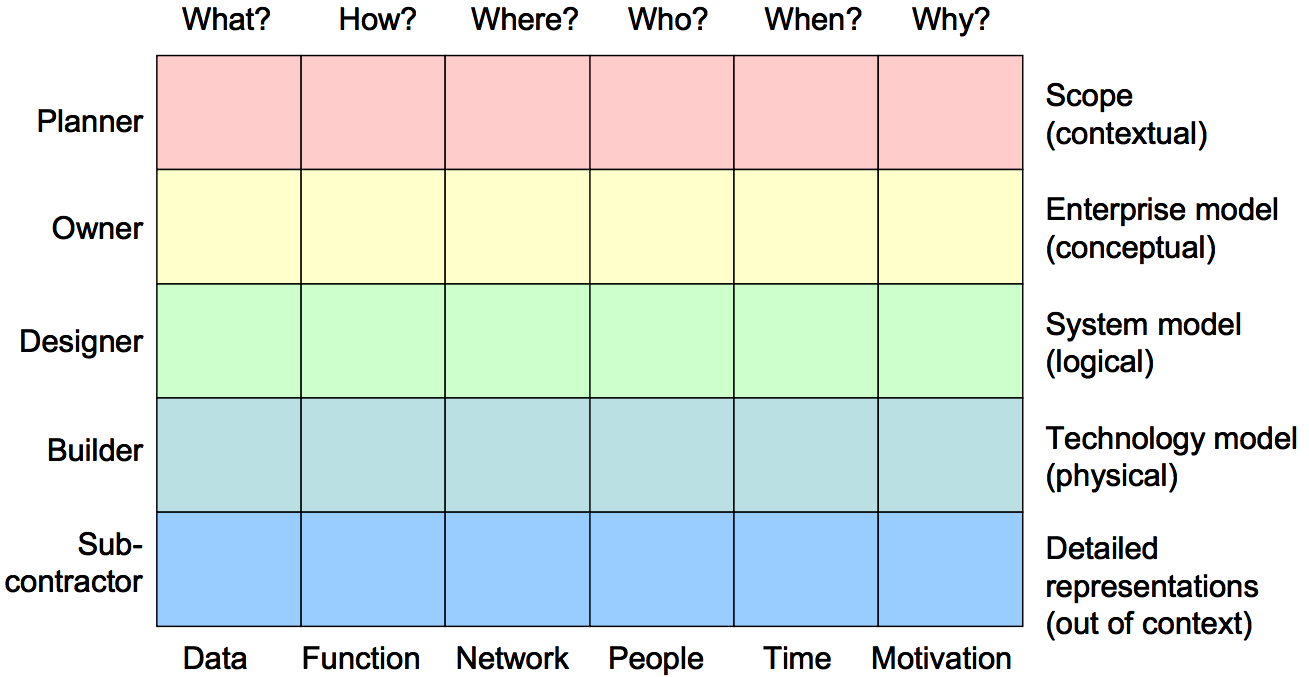
\includegraphics[width=1\textwidth]{images/Chapitre1/zachman.png}
 \end{center}
 \caption{TOGAF Architecture Development Method  \protect\cite{zachman1987framework}}
 \label{fig:Zachman}
\end{figure}

	\end{itemize}

Encore largement utilisé, le cadre Zachman est le premier à adresser l'entreprise dans son ensemble. Il est de plus facile à comprendre et ne dépend ni d'une méthode ou ni d'un outil en particulier. Sa mise en pratique est cependant fastidieuse à cause du grand nombre de cellules à modéliser. En outre, la mise en cohérence entre les différents artefacts n'est pas évidente car les relations entre les cellules n'est pas explicitement spécifiées. Le cadre Zachman offre un schemas de classification bien structuré mais ne spécifie aucune méthode pour mener les multiples activités d'architecture \cite{lankhorst2013enterprise}.


\item[TOGAF] \textit{(The Open Group Architectural Framework)}, le plus connu et le plus utilisé des cadres d'architecture \cite{winter2008enterprise}, est un standard de l'Open Group. TOGAF se compose essentiellement d'une architecture à quatre types points de vue~—~métier, information, applicatif et technique~—~et d'une méthode de conception~—~\textit{The Architecture Development Method (ADM)}. 

La méthode ADM correspond à un processus de conception cyclique. Elle préconise de piloter l'architecture d'une entreprise par la gestion des exigences. Les exigences sont dérivées de la stratégies et des objectifs métier de l'entreprise. Elles sont de ce fait considérées comme le centre névralgique des activités d'architecture et font le lien entre les différentes étapes, de la conception de l'architecture à sa mise en œuvre comme l'illustre la figure~\ref{fig:TOGAF}. 


\begin{figure}[!htbp]
 \begin{center}
  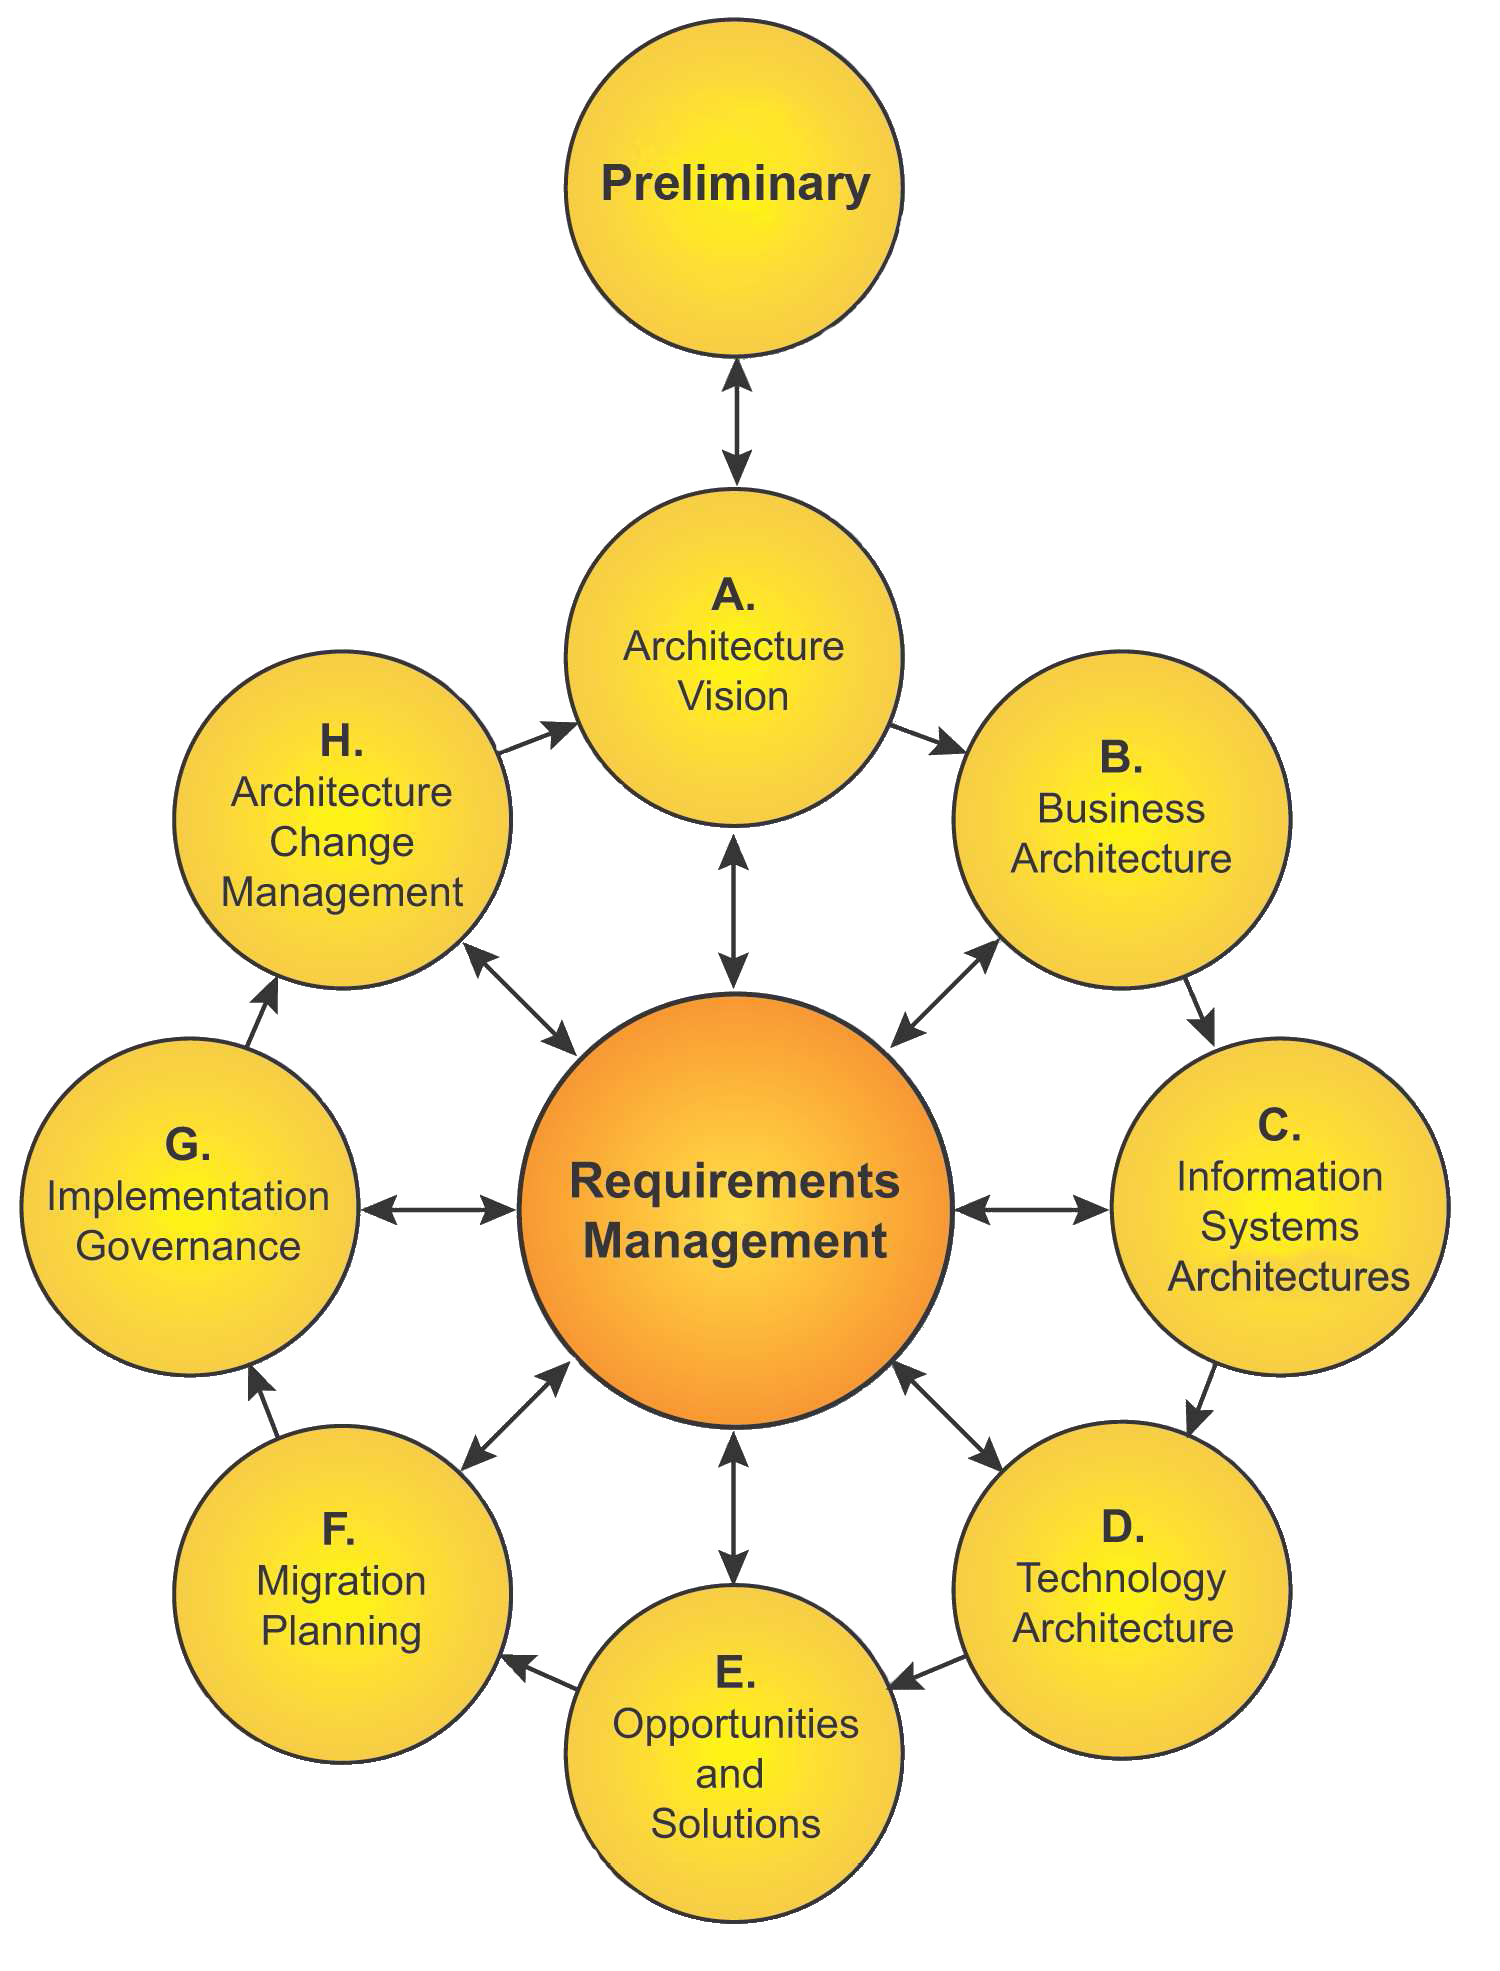
\includegraphics[width=0.8\textwidth]{images/Chapitre1/TOGAF9_Wheel.png}
 \end{center}
 \caption{TOGAF Architecture Development Method  \protect\cite{togaf2009}}
 \label{fig:TOGAF}
\end{figure}

La méthode ADM commence par une phase préliminaire qui correspond à l'initialisation ou encore la contextualisation de l'EA. Pendant cette phase, la disposition de l'entreprise à engager une démarche d'EA est évaluée et les grands principes d'EA sont définis en accord avec le métier. Le cycle ADM se poursuit avec les huit phases relatives à la création des vues métier, applicative, information et technique puis de planifier et de mettre en leur déploiement avant de les implémenter (notée de A à G). La dernière phase consiste à gérer les changements qui peuvent survenir suite aux évolutions métier ou technologiques pour assurer une mise à jour continue de l'architecture. 

Générique, TOGAF peut être appliqué à différents types d'organisation ou de secteurs d'activité. Flexible, il préconise  un ensemble de bonnes pratiques à adapter selon les cas. Il est par exemple possible de recourir au schéma de classification de Zachman dans le cadre d'une démarche ADM.

TOGAF comme Zachman laisse aux praticiens la liberté de choisir les langages de modélisation utilisés et le niveau de détail requis pour la conception des vues de l'architecture. 

\item[SGAM] \textit{(Smart Grid Architecture Model)} \cite{uslar2012standardization} adresse l'architecture du Smart Grid en englobant les trois domaines : SI, réseau électrique et réseau de télécommunication.  to be continued....

\item[Kruchten]

\item[RM-ODP]

\item[Archimate]

\item[•]



\end{description}


Les cadres d'EA n'utilisent pas tous les mêmes points de vue~: leurs nombres, leurs noms ainsi que les préoccupations qu'ils adressent varient. Néanmoins, ces 
frameworks recourent souvent, implicitement ou explicitement aux points de vue suivants~:

\begin{description}

\item[Point de vue métier]~:~ce point de vue reflète la vision métier de l'entreprise. On y retrouve ses objectifs métier de l'entreprise ainsi que ses processus. Les objectifs et les processus sont organisés par rapport la structuration de l'entreprise en termes d'acteurs internes et externes~;

\item[Point de vue fonctionnel]~:~ce point de vue organise l'entreprise en termes  de blocs fonctionnels implémentant des processus métier de l'entreprise. Cette structuration implique souvent une grande cohérence au sein d'un même bloc et une forte décorrélation entre blocs dans un souci de modularité et d'évolutivité. À l'échelle d'une entreprise, cette structuration devient vite complexe à cause du caractère étendu et transverse des processus métier impactés~;

\item[Point de vue applicatif]~:~ce point de vue structure l'entreprise en termes de blocs applicatifs. Chaque bloc implémente un ou plusieurs blocs fonctionnels. Il est aussi important de spécifier les échanges entre blocs applicatifs~;

\item[Point de vue technique] : ce point de vue correspond à l'infrastructure technique d'entreprise nécessaire à l'exécution des blocs applicatifs. Le point de vue technique spécifie ainsi les machines physiques et liens de communication utiles au déploiement des applications informatiques. 
\end{description}

En outre, ces cadres d'architecture sont orientés composants car ils utilisent des concepts tels que les macros processus, blocs fonctionnels ou encore les blocs applicatifs. Les informations sont modélisées soit implicitement et de manière diffuse à l'intérieur des vues (TOGAF), soit séparément dans une vue dédiée et décorrélée des autres vues (RM-ODP, Kruchten, SGAM).

De plus, ces frameworks organisent hiérarchiquement les différentes vues en appliquant \emph{« IT follows business »} comme principe : commencer par le point de vue métier et le dériver progressivement jusqu'à l'infrastructure technique déployée en passant par les fonctions et les applications \cite{winter2006essential}.


\section{Analyse en Architecture d'Entreprise}

La valeur ajoutée de l'architecture d'entreprise réside dans sa capacité à adresser le changement en offrant une vue holistique de l'entreprise. En effet, l'efficacité de l'entreprise  est garantie par une orchestration effective de ses différents composants et entités plutôt que par des optimisations locales et isolée \cite{nadler1992organizational}. 

La documentation et la description ne suffisent cependant pas à assurer une architecture qui soit à la fois cohérente et pertinente pour le métier. Les techniques d'analyse de modèles sont indispensables à l'optimisation globale et effectivement d'une architecture \cite{lankhorst2009enterprise}. Les techniques d'analyse de modèles jouent donc un rôle crucial dans tout processus de changement affectant l'entreprise en éclairant efficacement la prise de décision. En effet, l'analyse de l'architecture d'entreprise ne doit pas se résumer pas à la revue mentale ou manuelle d'une vue d'ensemble étant donnée la taille et la complexité des architectures impliquées.

	\subsection{Au-delà des modèles «~contemplatifs~»}

Les entreprises recourent aux frameworks d'EA pour les guider dans la création et la maintenance de leurs architectures et avoir ainsi une vue globale et cohérente de leurs stratégies, leurs processus métier et leurs IT.

Les artefacts issus d'une démarche d'EA se résument à un ensemble de documents utilisés comme supports de communication et comme schéma directeur au sein de l'organisation \cite{kulkarni_modelling_2013} \cite{clark_towards_2014}. Ces modèles fournissent certes un vocabulaire commun aux différentes parties prenanantes mais ne sont pas ni manipulables ni interprétables par une machine. Ce sont des modèles purement «~contemplatifs~». Cette terminologie est introduite par Bézivin en qualifiant les modèles de spécification utilisés pendant les premières phases de conception en génie logiciel. 

D'autres part, l'EA s'intéresse d'avantage aux aspects structuraux de l'entreprise. Pour cette raison, les modèles utilisés, bien qu'ils offrent l'abstraction nécessaire pour adresser la complexité de l'entreprise, sont le plus souvent statiques. Ce type de modèle ne permet pas d'appréhender les comportements de l'entreprise et sont donc insuffisants pour éclairer efficacement les prises de décision au niveau stratégique.

L'EA à travers les différents frameworks proposés lors de ces 30 dernières années a certes contribué à traiter de manière intégrée les différents aspects d'une entreprise tels que les processus, les personnel, les services et l'IT). Cependant la gestion des artefacts issus de l'EA reste un défi \cite{zachman1997enterprise} malgré l'existence d'outils sur étagère (Gartner Magic Quandrant). En effet, les architectes d'entreprise experts ainsi que les autres parties prenantes impliqués sont supposés utiliser leur bon jugement pour construire la bonne architecture. 

L'architecture créée est donc correcte par définition et dépend essentiellement des capacités de l'architecte et de son expertise. Certain travaux proposent de rentre l'EA plus ou moins dépendante à l'expertise d'une seule personne en utilisant en traduisant les représentations d'architecture en ontologies \cite{sunkle_analyzing_2013}. Les ontologies comme modèles exécutables permettent en effet de bénéficier des capacités d'analyse des raisonneurs disponibles 

Certaines méthodes d'EA sont accompagnés de langages de modélisation tel que Archimate. Dans leur quête de généricité, ces langages deviennent rapidement très larges et difficiles à manipuler. Les modèles produits sont d'autant plus difficiles à gérer qu'ils ne sont pas manipulables par une machine. L'activité d'analyse en EA, bien que cruciale, est donc compromise par toutes ces limitations. Cependant, des modèles et des techniques destinés à l'analyse des architectures d'entreprise existent mais l'analyse via des modèles exécutables reste encore marginale dans le domaine de l'EA \cite{kulkarni2013modelling}. 

Parmi ces travaux nous citons le framework LEAP \cite{clark2011leap}. C'est un framework léger et générique, complété d'un langage exécutable destiné à l'analyse des modèles issus de l'EA pour valider l'alignement des modèles métier et IT. 

Dans la section suivante nous discutons des différentes finalités de l'activité d'analyse et des diverses techniques employées.


	\subsection{Classification des approches d'analyse}
Lankhorst et al. \cite{lankhorst2009enterprise} classifie les différentes approches d'analyse d'architecture d'entreprise en quatre catégories selon deux dimensions (le type d'analyse et la technique emplyée) illustrées par la figure \ref{fig:classLankhorst}. La première dimension distingue entre deux types d'analyses d'architecture d'entreprise~:
	\begin{itemize}
		\item \textbf{l'analyse fonctionnelle} concerne les aspects fonctionnels de l'architecture. Elle permet par exemple de valider la structure ou de comprendre le comportement d'une architecture.
		\item \textbf{l'analyse quantitative} concerne les aspects non fonctionnels de l'architecture comme la performance ou le coût. 
\end{itemize}

\begin{figure}[!htbp]
 \begin{center}
  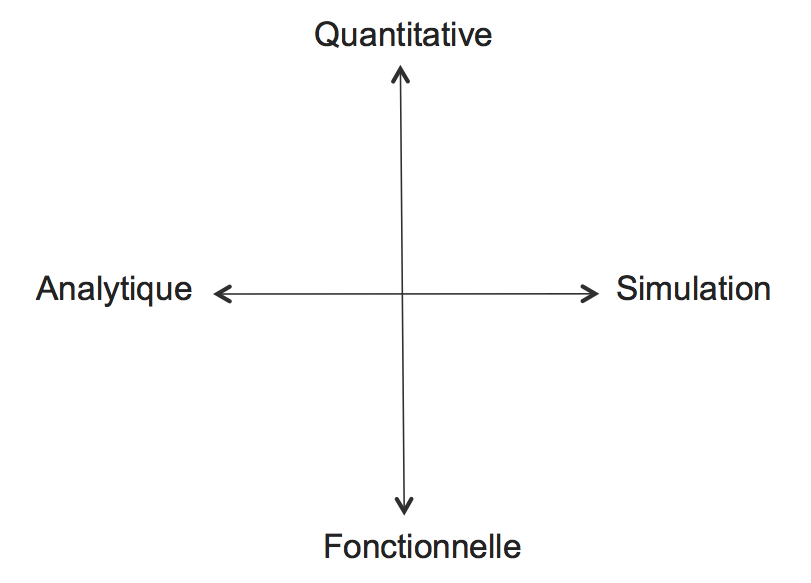
\includegraphics[width=0.75\textwidth]{images/Chapitre1/dimesionsLankhorts.png}
 \end{center}
 \caption{Classification des approches d'analyse selon Lankhorst et al. \protect\cite{lankhorst2009enterprise}}
 \label{fig:classLankhorst}
\end{figure}

La deuxième dimension distingue entre deux techniques pouvant être employées pour l'analyse fonctionnelle ou quantitative~:
	\begin{itemize}
		\item l\textbf{a technique de simulation} des modèles revient à exécuter ces modèles. La simulation dans le cas de l'analyse fonctionnelle est utilisée pour mieux appréhender les aspects dynamiques d'une architecture. La simulation quantitative permet de mesurer de paramètres quantitatifs tel que le temps d'exécution d'un processus métier par exemple à travers différentes itérations de la simulation. 
		\item \textbf{la technique analytique} est plus formelle que la simulation. Ici l'adjectif analytique signifie plutôt «~mathématique~» plus efficace que la simulation quantitative pour fournir des indicateurs de performance.  
	\end{itemize}
	
Ce schéma de classification offre un premier aperçu des différentes approches d'analyse d'architecture cependant il ne révèle pas toutes les variantes possibles et les subtilités d'une démarche d'analyse en architecture d'entreprise. Nous considérons donc les travaux de Buckl  et al. qui offre un système de classification plus détaillé. Ce système classification peut même être considéré comme un framework d'analyse d'architectures.

Contrairement à Lankhorst et al. \cite{lankhorst2009enterprise}, Buckl et al. \cite{buckl2009classifying} fait appel à cinq dimensions pour catégoriser les approches d'analyse d'architecture. Ces dimensions de classification sont illustrés par la figure~\ref{fig:classBuckl}. Nous les détaillons dans la suite du manuscrit.

\begin{figure}[!htbp]
\begin{tikzpicture}
  \hspace*{-1cm}
  \path[mindmap,concept level 1/.append style={level distance=4cm}]
    node[concept, scale=0.7] {L'analyse en Architecture d'Entreprise}
    [clockwise from=0]
    child[concept color=black] {
      node[concept, scale=0.9] {Sujet de l'analyse}
      [clockwise from=60]
      child { node[concept, scale=0.9] {Structure} }
      child { node[concept, scale=0.9] {Dynamique} }
      child { node[concept, scale=0.9] {Statistiques} }
    }
    child[concept color=black] {
      node[concept, scale=0.9] {Référence temporelle}
      [clockwise from=-30]
      child { node[concept, scale=0.9] {Ex post} }
      child { node[concept, scale=0.9] {Ex ante} }
    }
    child[concept color=black] { 
    	  node[concept, scale=0.9] {Techniques} 
      [clockwise from=-60]
      child { node[concept, scale=0.9] {Basée sur les experts} }
      child { node[concept, scale=0.9] {À base de règles} }
      child { node[concept, scale=0.9] {À base d'indicateurs} }
    }
    child[concept color=black] { 
      node[concept, scale=0.9] {Préoc\-cupations}
      [clockwise from=-150]
      child { node[concept, scale=0.9] {Fonction\-nelles} }
      child { node[concept, scale=0.9] {Non Fonctionnelles} }
    }
    child[concept color=black] { 
    	  node[concept, scale=0.9] {Auto\-référentialité}
      [clockwise from=-180] 
      child { node[concept, scale=0.9] {Aucune} }
      child { node[concept, scale=0.9] {un niveau} }
      child { node[concept, scale=0.9] {plusieurs niveaux} }      
    }; 
       
\end{tikzpicture}

\caption{Classification des approches d'analyse selon Buckl et al. \protect\cite{buckl2009classifying}}
 \label{fig:classBuckl}
\end{figure}


	\begin{description}
	\item \textbf{Sujet de l'analyse} 

L'analyse se porte sur trois aspects différents de l'architecture~:~sa structure, son comportement dynamique ou son comportement statistique. L'analyse de la structure est nécessaire étant la complexité des entreprises. Celle-ci est due à la densité des interconnexions entres ses composants. La complexité de la structure induit aussi une complexité au niveau de son comportement d'où la nécessité d'analyser l'aspect comportemental de l'architecture pour évaluer l'impact d'une anomalie le déroulement d'un processus par exemple. De plus, l'analyse et l'agrégation des mesures statistiques provenant du comportement offrent une meilleure compréhension de l'architecture.

	\item \textbf{Référence temporelle}

L'architecture peut se porter sur l'architecture d'une entreprise dans son état courant ou telle qu'elle est planifiée. Une analyse ex post concerne les modèles d'une architecture implémentée alors qu'une analyse ex ante se réfère à différents scénarios élaborés pour une futur implémentation.

	\item \textbf{Technique d'analyse}

Les techniques d'analyse peuvent se baser sur des experts, sur des règles ou sur des indicateurs. Les approches d'analyse orientée experts sont les moins formelles dépendent du niveau d'expertise de la personne impliquée et nécessitent plus de temps mais elle sont aussi les plus flexibles. Les résulats d'une telle analyse prennent la forme de conseils concrets ou d'idées générales pour l'architecture en question.

Les techniques d'analyse basées sur des règles sont plus formelles que celles basées sur les experts et peuvent être plus facilement automatisées. Ces règles décrivent des modèles de conceptions que l'architecture doit respecter ou éviter. 

Les techniques d'analyse basées sur des indicateurs sont encore plus formelles que les deux précédentes et servent à évaluer en les quantifiant certaines propriétés de l'architecture. Les résultats d'une telle analyse doivent cependant être interprétés avec prudence. Elle sont en effet basés sur des hypothèses souvent sujettes à évoluer.

	\item \textbf{Préoccupations de l'analyse}

De même que la classification de Lankhorst, Buckl fait la différence entre les analyses fonctionnelles et non fonctionnelles. L'analyse fonctionnelle évalue si l'architecture remplie les fonctions métier de l'entreprise telles la production ou la vente. Il est toutefois aussi important d'évaluer des aspects non fonctionnels tels que le temps d'exécution d'un processus ou le coût de l'implémentation ou de maintenance d'une architecture. Contrairement à Lankhorst, Buckl emploie le terme \textit{non fonctionnelle} plutôt que \textit{quantitative} en arguant que certains aspects non fonctionnels telle que la sécurité peuvent être analysés de manière non quantitative.  

	\item \textbf{Autoréférentialité}
	
Les personnes responsables de l'architecture d'entreprise peuvent faire partie l'architecture créée car elle font aussi partie de l'entreprise. Qui plus est, l'activité de décrire et planifier l'architecture de l'entreprise peut elle-même être décrite et planifiée et fait par conséquent partie de l'activité d'architecture d'entreprise. Selon Buckl \cite{varela1974autopoiesis} l'entreprise est en effet un système vivant capable de faire sa propre autopsie \cite{varela1974autopoiesis}.
L'analyse peut considérer un seul niveau d'autoréférentialité en intégrant les activités de management d'architectures. Une analyse à plusieurs niveaux d'autoréférentialité incorporent des activités de meta-management d'architetcure comme par exemple la gouvernance des activités de management d'architectures.
L'autoréférentialité augmente la complexité d'analyse. Peu de travaux considèrent des niveaux d'autoréférentialité  multiples \cite{smook2014executable}. Nous citons parmis celle-ci les travaux de \cite{metrailler_evolis_2014} qui traitent la gestion et la gouvernance d'architectures notamment en définissant des stratégies d'évolution des architectures actuelles vers les architectures cible dans un framework dédié. 

\end{description}

	\subsection{Analyse de la structure}
	Le moteur essentiel de l'EA est d'arriver à aligner l'infrastructure informatique de l'entreprise avec ses processus métier \cite{lankhorst2013enterprise}. afin d'en améliorer l'efficacité et de maximiser ainsi ses bénéfices. L'alignement Business/IT reste une problématique majeure et cruciale pour les entreprises qui s'appuient sur les technologies de l'information pour réaliser leurs objectifs métier \cite{kaisler_enterprise_2005}. Zachman affirment même que seules les entreprises capables d'aligner rapidement leurs SI à leurs stratégies métier sont en mesure de survivre dans un environnement hautement concurrentiel \cite{zachman1997enterprise}.
	
	Pour \cite{lankhorst2013enterprise} l'EA a pour vocation de décrire une telle organisation en offrant une vue générale et homogène de son métier, de son patrimoine applicatif, de son infrastructure technique ainsi que de leur évolution pour en faciliter l'analyse par biais d'un ensemble cohérents de principes, méthodes et modèles. En plus d'offrir cette vision globale de l'entreprise, et  l'EA explicite et documente les relations entre les procesus métier et l'IT de l'entreprise \cite{kaisler_enterprise_2005}. 
	
	En offrant ainsi une vision globale de l'entreprise et en documentant les relations entre ses différents composants, l'EA est un instrument incontournable pour les architectes dans leur démarche d'alignement Business/IT. Cependant, les méthodes et techniques actuelles ne suffisent pas à atteindre cet objectif \cite{barn2013enterprise}. 
	
	Le premier verrous identifié est lié à la dynamique des entreprises actuelles. Les processus métier, les technologiques, les structures organisationnelles, de même que l'environnement sont en constante évolutions. Les changements sont si rapides et nombreux qu'un réel alignement est d'avantage un vieux pieux \cite{lankhorst2013enterprise}. L'alignement entre métier et IT est plutôt un idéal kantien vers lequel l'entreprise doit tendre à défaut de le réaliser complètement.
	
	Le second verrous relève de la discipline même d'architecture tenant d'avantage de l'art que de la science. En effet, l'architecte d'entreprise analyse souvent de la documentation (tels que des tableurs Excel ou des illustration Power Point) même si quelques logiciels permettent désormais de visualiser ces modèles. Cette tâche devient vite ardue dans le cas des très grandes entreprises dont l'important patrimoine applicatif ressemble à un plat de spaghetti.
	
	Les modèles peuvent aider les architectes dans leurs démarches pour surmonter les verrous cités précédemment. D'une part, les modèles exécutables augmentent l'agilité de l'architecture par exemple en détectant automatiquement les incohérences dès les premières phases de conception. Les approches de modélisation recourent souvent à des langages semi-formels qui ne permettent pas de vérifier dynamiquement et automatiquement certaine propriétés de l'architecture conçue comme la cohérence entres vues. 
	
	Partant de ce constat, \cite{sunkle_analyzing_2013} proposent de recourir aux ontologies tirant ainsi des raisonneurs disponibles pour analyser la structure des architecture d'entreprise. Ils arrivent ainsi à mener des analyses quant à l'impact du changement ou encore les relations et dépendances entre les opérations métier et les applications informatiques de l'entreprise. Cependant, les ontologies ne sont pas des technologies familières aux architectures d'entreprise plus habitués aux diagrammes UML par exemples. Elles nécessitent de plus une traductions des modèles d'architectures vers une représentation en terme d'ontologies engendrant un gap sémantiques entre les modèles utilisés pour la représentation et les ontologies utilisées pour l'analyse.
	
	Afin d'assister différent acteurs impliquer dans l'EA comme l'architecte d'entreprise, le manager ou encore l'ingénieur IT, \cite{bruneliere2013support} proposent de créer un modèle de mapping où sont représentées les liens entre des modèles hétérogènes (tels que des tableurs Excel ,de la documentation ou des bases de données) en utilisant des modèles manipulables par machine et en mettant à profit les techniques de tissages de modèles issus de l'IDM. Ces travaux adresse l'hétérogénéité des modèles manipulés et offre une vue intégrée de l'architecture globale de l'entreprise en l'adaptant aux acteurs concernés. Mais elle ne permet pas de mener des analyses concernant l'impact du changement par exemple.   

	
	\subsection{Analyse du comportement}
	\subsubsection{Finalités}
	Pour Shannon \cite{shannon1975systems}, la simulation est 
«~\emph{un processus consistant à modéliser un système réel et à mener des expérimentations sur le modèle obtenu dans le but de comprendre le comportement du système et/ou d'évaluer différentes stratégies concernant son fonctionnement}~». 
Quel qu'en soit le domaine d'application, la simulation est un moyen d'apprécier les choix des concepteurs sur le comportement du système modélisé. Elle se traduit par exemple par l'animation d'un modèle (représentant notre perception du système, qu'il soit existant ou à construire) et l'étude du comportement de ce modèle en fonction des variables en entrée.  

La simulation des architectures d'entreprise permet aux architectes d'entreprise de modifier des stratégies localement et d'observer l'impact de ces modification sur le comportement globale du système \cite{2008towards}. La simulation des architectures d'entreprise est d'autant plus cruciale dans le contexte des Smart Grids. Ces derniers sont en constante et rapide transformation~:~évolution des cadres législatifs,  apparition de nouveaux partenaires, hétérogénéité des interactions avec les clients finaux via les compteurs intelligents, Internet, les téléphones ou encore les tablettes. 

Ainsi, le recours à la simulation dès les premières phases du cycle de vie des SI des Smart Grids augmente leur évolutivité en apportant une aide supplémentaire à leur validation. La simulation des modèles facilite leur exploration  par les experts métier et lève les ambiguïtés engendrées par les modèles purement contemplatifs. Elle permet en outre un prototypage rapide et une analyse itérative des modèles par les parties prenantes tels que les architectes d'entreprise, les expert métier, les analystes ou les architectes IT.

	\subsubsection{Approches de simulation existantes et leurs limites}
	Il existe plusieurs approches pour l'analyse d'architecture d'entreprise. \cite{manzur2015xarchimate} en recensent quatorze et les classent selon les quatre dimension du schéma de classification de Lankhorst (précédemment illustré par la figure \ref{fig:classLankhorst}). Seulement quatre approches parmi les quatorze recourent à la simulation comme outil d'analyse d'une architecture d'entreprise.

Le nombre limité d'approches utilisant la simulation pour l'analyse d'architecture d'entreprise est due au fait que l'EA est initialement conçue comme une description statique des composants essentiels de l'entreprise et de leurs interconnexions \cite{hoffman2013enterprise}. Les cadres d'EA standards ne comprennent en effet pas les informations nécessaires pour analyser les aspects comportementaux d'une entreprise et mettent d'abord l'accent sur ses aspects structuraux tels que les liens entre les processus et les applications métier. Il en résulte que les outils d'EA n'adressent souvent que les aspects statiques de l'entreprise car ils se basent sur les mêmes cadres d'EA.

%\cite{buckl2009classifying} classifient les approches d'analyse d'architecture existantes selon leur propre système de classification illustré par la figure \ref{fig:classBuckl}. Nous rapportons cette classification dans le tableau après l'avoir mis à jour en l'enrichissant avec d'autres approches recourant à la simulation. Nous tirons le même constat que pointe l'état de l'art de \cite{manzur2015xarchimate}. 

Nous nous intéressons donc aux travaux qui considère la dimension dynamique d'une architecture d'entreprise comme sujet d'analyse. Parmi ces approches, celles développées par \cite{glazner2011enterprise}, \cite{ludwig2011organizational} et \cite{manzur2015xarchimate} soulignent l'importance d'analyser en le simulant le comportement d'une architecture d'entreprise. 

\cite{glazner2011enterprise} propose une approche de simulation hybride pour évaluer le comportement d'une entrepris en combinant une simulation à événements discrets et une simulation multi-agents. \cite{glazner2011enterprise} met à profit les capacité d'abstraction de l'EA pour adresser la complexité d'un système telle que l'entreprise et s'en sert comme socle pour structurer les modèles de simulation. Cette approche est limitée par le fait que les techniques et les langages utilisés pour la simulation sont décorrélés des langages de représentation utilisés par les architectes d'entreprise entrainant ainsi un gap sémantique entre l'aspect statique de l'entreprise (les composants de l'entreprise et leurs relations) et son aspect dynamique (le comportement des composants).  

\cite{ludwig2011organizational} simulent une architecture d'entreprise selon la configuration organisationnelle d'une entreprise. Ils développent ainsi un langage exécutable pour décrire les relations entre des concepts de l'ordre organisationnels tels qu'une entité de l'entreprise, le rôle qu'elle joue, les services qu'elle procure et les processus dans lesquels elle intervient. Les modèles sont ensuite exécutés. La méthode et l'outil développé permettent de reconfigurer les modèles organisationnels lors de l'exécution. Ces travaux n'adressent cependant que la vue métier et une partie de la vue fonctionnelle d'une architecture d'entreprise.

\cite{manzur2015xarchimate} proposent une plateforme de simulation qui s'appuie sur deux métamodèles différents~:~un premier métamodèle correspondant au langage Archimate pour spécifier les composants structurels de l'architecture et un deuxième métamodèle complémentaire pour spécifier les comportements des composants structurels. Les modèles sont ensuite simulés afin d'observer le comportement de l'architecture et de l'évaluer selon les indicateurs établis. Cependant cette approche évalue uniquement les aspects non fonctionnels d'une architecture d'entreprise.



%La modélisation c'est pour abstraire
%Pour simuler on a besoin de détails 
%\cite{de2005enterprise} : dynamique par xlm  



\section{Ingénierie Dirigée par les Modèles}

L'Ingénierie Dirigée par les Modèles (IDM) est née du constat que le paradigme 
du « tout est objet », prôné dans les années 1980, a atteint ses limites avec ce 
début de siècle \cite{greenfield2004software}. En effet, face à la croissance de 
la complexité des systèmes logiciels, au coût de la main d'œuvre et de 
maintenance, une approche centrée sur le code, jugé alors seul représentant 
fiable du système, suscitait de moins en moins l'adhésion des industriels et du 
milieu académique. 

Partant de ce constat, l'Object Management Group (OMG) a proposé en novembre 
2000, l'approche MDA (Model Driven Architecture) qui s'inscrit dans le cadre 
plus général de l'IDM et se réalise autour d'un certain nombre de standards tels 
qu'UML, MOF, XML, QVT, etc. Le monde de la recherche s'y est aussitôt intéressé 
pour dégager les principes fondamentaux de l'IDM 
\cite{bezivin2001towards}\cite{kent2002model} \cite{de2002using} et déjouer le 
piège des définitions parfois trop floues qui prêtent à confusion entre les 
concepts liés aux paradigmes d'objet et de modèle \cite{bezivin2004search}. Par 
ailleurs, des industriels comme IBM \cite{booch2004mda} et Microsoft 
\cite{greenfield2004software} ont aussi rendu publiques leur vision de l'IDM. 
Ainsi, l'IDM prend son origine dans la convergence de toutes ces visions et des 
avancées techniques de chacun.

L'originalité de l'IDM ne réside pas dans le recours systématique aux modèles 
dans le développement logiciel comme le laisserait entendre sa terminologie  
\cite{bezivin2004rapport}. Plusieurs méthodes de modélisation telles que Merise 
ou SSADM préconisent aussi l'utilisation de modèles dont le rôle s'achève aux 
phases amont du développement logiciel : l'analyse et la conception. Les modèles 
servent alors à faciliter la communication et compréhension entre les différents 
acteurs mais n'interviennent pas dans la phase de production, de maintien et 
d'évolution. Nous parlons dans ce cas de modèles « contemplatifs ». 

L'IDM a pour objectif de rendre les modèles « productifs » sur tout le cycle de 
vie du système et à tout niveau d'abstraction. Pour y parvenir, les modèles 
doivent être décrits formellement pour être interprétés et exécutés par une 
machine. Dès lors, ces modèles permettent d'industrialiser la production 
logicielle, jusque-là centrée sur le code produit par l'informaticien 
\cite{bezivin2005unification}.

En mettant à profit des disciplines comme la modélisation par objets, 
l'ingénierie des langages, la compilation de langages, les méthodes formelles, 
la programmation par composants, etc., l'IDM offre un cadre intégrateur reposant 
sur quelques concepts fondamentaux : la notion de modèle et la relation 
\textit{ReprésentationDe}, la notion de métamodèle et la relation 
\textit{ConformeÀ}.

\subsection{Concepts et relations de l'IDM}
\subsubsection{Modèle et ReprésentationDe}
La notion de modèle est centrale dans l'IDM car, comme nous venons de voir, 
l'enjeu de cette approche est de rendre les modèles productifs sur tout le cycle 
de vie du système. Il n'existe pas de définition universelle de la notion de 
modèle. En nous appuyant sur les définitions données dans les travaux 
\cite{minsky1967computation} \cite{bezivin2001towards} et 
\cite{seidewitz2003models}, nous adoptons la définition suivante du terme modèle 
:

\begin{definition}
Un modèle est une abstraction d'un système, selon le bon point de vue, qui 
permet de répondre à des questions prédéfinies sur ce système en lieu et place 
de celui-ci.
\end{definition}

De cette définition découle la première relation fondamentale de l'IDM qui lie 
le modèle et le système qu'il représente. Celle-ci est nommée 
\textit{ReprésentationDe} et notée $(\mu)$. Bien que la relation 
\textit{ReprésentationDe} ne soit pas nouvelle dans l'ingénierie logicielle 
(Merise, UML), l'IDM a permis d'en définir les contours \cite{atkinson2003model} 
\cite{seidewitz2003models} \cite{bezivin2004search}.

\begin{figure}[!htbp]
 \begin{center}
  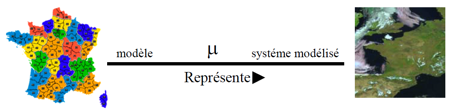
\includegraphics[width=1\textwidth]{images/Chapitre1/favresystememodele.png}
 \end{center}
 \caption{Relation entre système et modèle \protect\cite{favre2006ingenierie}}
 \label{fig:systemModele}
\end{figure}

Cette définition n'est pas restreinte à l'informatique et pourrait s'appliquer à 
n'importe quel système. 
La figure~\ref{fig:systemModele} reprend l'exemple connu de la cartographie où 
une carte géographique joue le rôle de modèle pour une région donnée jouant 
alors le rôle de système modélisé. 

L'intérêt de l'IDM est de produire des modèles exploitables informatiquement. 
Ceci n'est possible que si ces modèles sont décrits par des langages formels. Il 
devient alors important de bien définir ces langages à l'aide de métamodèles

\subsubsection{Métamodèle et ConformeÀ}
L'originalité de l'IDM ne réside pas dans la relation ReprésentationDe qui 
trouve plutôt son origine dans les méthodes de modélisation telles que Merise ou 
SSADM. L'apport de l'IDM est dans l'utilisation systématique de métamodèles pour 
la description des langages de modélisation. 

Il existe plusieurs définitions de la notion de métamodèle dans la littérature. 
Cependant la définition suivante est communément admise 
\cite{bezivin2004rapport}.

\begin{definition}
Un métamodèle est un modèle du langage de modélisation qui sert à exprimer les 
modèles.
\end{definition}
Une autre définition courante mais erronée de la notion de métamodèle suppose 
qu'un métamodèle est un modèle d'un modèle. La figure~\ref{fig:modelofmodel} 
reprend l'exemple de la cartographie évoquée plus haut. Nous appliquons 
récursivement la relation \textit{ReprésentationDe} $(\mu)$ au territoire 
français. Ici une carte de la France joue le rôle de modèle du territoire 
français et un fichier XML joue le rôle de modèle de la carte. Dans ce contre 
exemple, le fichier XML n'est pas un métamodèle de la France. Un métamodèle 
n'est donc pas un modèle d'un modèle.

\begin{figure}[!htbp]
 \begin{center}
  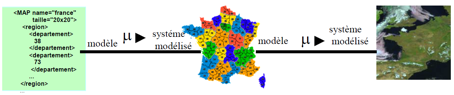
\includegraphics[width=1\textwidth]{images/Chapitre1/modelofmodel.png}
 \end{center}
 \caption{Modèle de modèle selon l'exemple de la cartographie 
\protect\cite{favre2006ingenierie}}
 \label{fig:modelofmodel}
\end{figure}

Par ailleurs, le concept de métamodèle induit la deuxième relation fondamentale 
de l'IDM liant un modèle à son métamodèle. Cette relation est nommée 
\textit{ConformeÀ} et notée $\chi$ \cite{bezivin2004search} 
\cite{favre2004towards}. La figure \ref{fig:carteFavre} reprend l'exemple de la 
cartographie où la légende de la carte joue le rôle de métamodèle ($\chi$) pour 
une carte de la France. En effet, pour être lisible, la carte doit être conforme 
à la légende.

\begin{figure}[!htbp]
 \begin{center}
  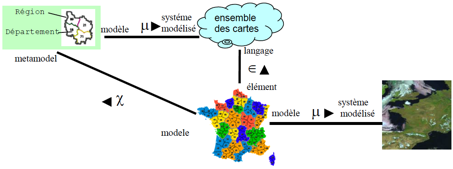
\includegraphics[width=1\textwidth]{images/Chapitre1/cartecompleteIDM.png}
 \end{center}
 \caption{Relations entre système, modèles, métamodèle et langage de 
modélisation \protect\cite{favre2006ingenierie}}
 \label{fig:carteFavre}
\end{figure}

\subsection{Transformation de modèle}
Dans la partie précédente, nous avons introduit les concepts fondamentaux de 
l'IDM que représentent la notion de modèle et la relation 
\textit{ReprésentationDe} ainsi que la notion de métamodèle et la relation 
\textit{ConformeÀ}. Comme expliqué, la préoccupation majeure de l'IDM est de 
rendre les modèles opérationnels sur tout le cycle de vie des systèmes 
logiciels, depuis l'analyse et la conception jusqu'à la maintenance et 
l'évolution. Ainsi, la transformation de modèle se retrouve au cœur de l'IDM car 
c'est à travers elle que se fait l'automatisation des traitements apportés aux 
modèles. Nous allons d'abord donner une définition de la notion de 
transformation de modèle puis en présenter les types et les usages.

\subsubsection{Définition de la transformation de modèle}
L'OMG définit une transformation de modèle comme «~le processus consistant à 
convertir un modèle en un autre modèle d'un même système~» \cite{omg2011meta}. 

\cite{kleppe2003mda} proposent une définition moins générique en insistant sur 
l'aspect automatique de ce processus, ainsi, «~une transformation de modèle 
consiste en la génération automatique d'un modèle source en un modèle cible, 
selon une description établie de cette transformation~». Cette définition 
implique aussi qu'une transformation est décrite à un plus haut niveau 
d'abstraction : au niveau d'un métamodèle auquel elle doit se conformer. 

\cite{mens2006taxonomy} étendent cette définition en considérant qu'une 
transformation est une opération qui peut avoir en entrée un ou plusieurs 
modèles source et en sortie un ou plusieurs modèles cible~: 

\begin{definition}
Une transformation génère automatiquement un ou plusieurs modèles cible à partir 
d'un ou plusieurs modèles source, selon une description établie de la 
transformation. 
\end{definition}

C'est cette dernière définition que nous allons adopter dans ce document. Par 
ailleurs, notons que, si les métamodèles source et cible sont différents, la 
transformation est dite exogène. Si les métamodèles source et cible 
correspondent au même métamodèle, la transformation est dite endogène. Ces 
termes ont été introduits par \cite{mens2006taxonomy}.

\subsubsection{Composants d'une transformation de modèle} 
La figure \ref{fig:composantTransfo} illustre les composants d'une 
transformation de modèle~:~les modèles source, les modèles cible, la définition 
de la transformation et le moteur qui va opérer la transformation selon sa 
définition. 

La description de la transformation spécifie comment un ou plusieurs modèles 
source sont transformés en un ou plusieurs modèles cible. Elle est écrite dans 
un langage de transformation de modèle. Par exemple, si c'est un langage à base 
de règles, la description de la transformation consiste en un ensemble de règles 
de transformation à opérer \cite{kleppe2003mda}. 

Un moteur de transformation exécute ou interprète la description. Il applique 
donc la description aux modèles source pour produire les modèles cible en 
suivant les étapes ci-dessous \cite{tratt2005model}~:

\begin{itemize}
\item Identifier l'élément du ou des modèles source à transformer.
\item Pour chaque élément identifié, produire l'élément cible qui lui est 
associé dans le ou les modèles cible.
\item Produire une trace de la transformation qui lie les éléments du ou des 
modèles cibles aux éléments du ou des modèles source.
\end{itemize}

\begin{figure}[!htbp]
 \begin{center}
   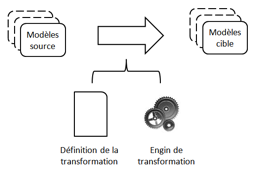
\includegraphics[width=0.7\textwidth]{images/Chapitre1/composanttransfo.png}
 \end{center}
 \caption{Composants d'une transformation de modèle}
 \label{fig:composantTransfo}
\end{figure}

\subsubsection{Usages de la transformation de modèles }
Les transformations de modèles sont au cœur d'une démarche dirigée par les 
modèles~:~elles permettent d'automatiser les manipulations subies par les 
modèles telles que la modification, la création, l'adaptation, la composition ou 
encore le filtrage de modèles, à travers la réutilisation systématique 
d'informations contenues dans les modèles existants. 

Il est possible de recourir aux transformations de modèles sur tout le cycle de 
vie d'un système. Les usages les plus répondus sont le raffinement, 
l'intégration d'outils, la composition, l'analyse, la simulation et 
l'optimisation que nous présentons dans la suite de ce document. 

\begin{description}

\item \textbf{Raffinement}

Le raffinement consiste à rajouter plus de détails au modèle initial. Ce type de 
transformation peut aussi bien être endogène (métamodèles source et cible 
identique) ou exogène (métamodèle source et cible différents). Le raffinement se 
prête parfaitement à toute la partie descendante du cycle en V où les modèles 
passent à des niveaux d'abstraction plus bas. Ceci revient à faire des 
transformations successives de type modèle-à-modèle et une transformation de 
type modèle-à-texte pour aboutir au code final.

Raffiner un modèle revient à décomposer des concepts de haut niveau, à choisir 
un algorithme particulier, à spécialiser un concept pour un contexte donné ou 
encore à le concrétiser sous forme d'une solution exécutable par une machine en 
générant le code à partir de modèles de plus haut niveau d'abstraction 
\cite{czarnecki2000intentional}. 

\item \textbf{Intégration d'outil}

Il existe une panoplie d'outils disponibles pour créer, manipuler, analyser ou 
encore simuler des modèles. Souvent ces outils utilisent des métamodèles 
internes et des espaces techniques qui leurs sont propres. Ainsi, l'échange de 
modèle entre ces outils est compromis et l'interopérabilité est fortement 
entravée. L'utilisateur se trouve obligé d'utiliser un seul et même outil sur 
tout le cycle de vie du système et ne peut donc pas tirer avantage des 
possibilités offertes par d'autres outils plus adaptés à ses besoins à certaines 
étapes.

L'intégration d'outil est une solution pour palier la divergence syntaxique et 
sémantique des outils et des langages de modélisation par le biais la 
transformation de modèle \cite{tratt2005model}. Ce type de transformation permet 
de naviguer entre deux métamodèles, de synchroniser des modèles qui évoluent 
séparément sur des outils distincts, de faire des mapping entre métamodèles pour 
maintenir la cohérence des modèles conformes à ces métamodèles. Il sera donc 
possible de faire appel à des outils mieux adaptés à chaque étape du cycle de 
vie.

\item \textbf{Composition}

Pour réduire la complexité inhérente à la modélisation et à l'analyse de grands 
systèmes, tels que les Smart Grids par exemple, il est possible d'adopter une 
approche par points de vue qui permet de séparer les préoccupations. Les modèles 
produits correspondent donc à ces différents points de vue qu'on peut ainsi 
valider séparément dans un premier temps. A l'issue de cette approche modulaire, 
on pourra composer ces modèles, c'est-à-dire les assembler, pour aboutir un 
modèle global du système.

Dans le cas le plus simple, les deux modèles à composer sont conformes à un même 
métamodèle. Cependant, il est aussi possible de composer deux modèles conformes 
à deux métamodèles différents. 

Les deux modèles à composer peuvent aussi présenter des concepts en commun. Deux 
techniques existent pour composer des modèles, que nous illustrons dans la 
figure \ref{fig:compoExemple}~:

\begin{itemize}
\item La première technique consiste à les fusionner. Dans ce cas, le modèle 
final résultant de la composition doit contenir toutes les informations issues 
des modèles initiaux, sans duplication des informations communes 
\cite{bezivin2006canonical}.
\cite{fleurey2008generic} présente un framework générique capable de composer 
des modèles indépendamment de leurs langages de modélisation. L'approche 
consiste à identifier les éléments qui représentent le même concept dans les 
deux modèles à composer et à les fusionner dans un nouveau modèle qui représente 
une vue intégrée de ces concepts. Il est aussi possible de spécialiser le 
framework pour un métamodèle particulier mais qui reste conforme au MOF.

\item La deuxième technique consiste à les tisser. Dans ce cas, on crée des 
correspondances entre les éléments qui représentent un même concept. Un 
métamodèle générique est créé pour définir les correspondances qui sont donc 
modélisées dans le modèle final. On y retrouve donc les éléments en commun 
dupliqués mais liés par un lien de correspondance. 
\end{itemize}

Il est à noter que le modèle issu du tissage de deux modèles $M_{A}$ et $M_{B}$ 
peut être utilisé comme modèle intermédiaire que l'on note $M_{T}$ pour la 
fusion de $M_{A}$ et $M_{B}$. Dans ce cas L'opération de fusion consiste à 
produire un modèle $M_{AB}$ en prenant comme entrée $M_{A}$, $M_{B}$ et $M_{T}$. 
Cette technique est notamment utilisée par \cite{del2007semi} pour la 
composition semi-automatique de modèles.

\begin{figure}[!htbp]
 \begin{center}
  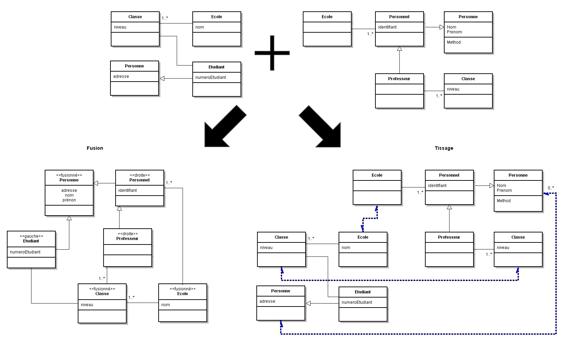
\includegraphics[width=1\textwidth]{images/Chapitre1/compoExemple.png}
 \end{center}
 \caption{Exemple de composition de deux modèles}
 \label{fig:compoExemple}
\end{figure}

\item \textbf{Simulation}

La transformation de modèle peut être utilisée pour simuler des modèles. En 
effet, une transformation de modèle peut mettre à jour le système modélisé. Dans 
ce cas, le modèle cible est une mise à jour du modèle source et la 
transformation est de type sur-place (modèles source et cible confondus). 

Par exemple, \cite{syriani2011multi} simule un comportement simple d'un jeu de 
Pacman en utilisant la transformation de modèle. La transformation spécifie les 
règles de transition qu'une instance du jeu peut prendre (Pacman et fantôme se 
trouvant dans la même case, Pacman et pomme se trouvant dans la même case, 
etc.). En ingénierie des langages, ceci revient à définir la sémantique 
opérationnelle d'un langage de modélisation. L'exécution de la transformation 
anime le modèle en fonction du comportement qu'on lui confère.

La transformation peut aussi être utilisée comme intermédiaire dans la 
simulation de modèle. Des modèles en entrée d'un outil de simulation externe 
sont produits par une transformation des modèles qu'on souhaite simuler. Cette 
technique permet de tirer profit d'outils de simulation existant sur le marché 
en utilisant l'intégration d'outils.

\item \textbf{Analyse et optimisation}

La transformation de modèle peut être utilisée pour les activités d'analyse de 
modèle. Une analyse simple telle que le calcul de métrique de similarité entre 
deux modèles via la transformation de modèle est donnée dans \cite{del2007semi} 
avec un modèle de transformation écrit en ATL \cite{jouault2006transforming}. 

Des analyses plus complexes sont possibles grâce à l'intégration d'outils 
d'analyse externes vers lesquels les modèles source sont transformés.

\cite{biehl2010integrating} propose d'utiliser la transformation de modèle pour 
l'analyse de sûreté de fonctionnement dans le domaine de l'automobile. Les 
modèles source sont transformés en modèles conformes au métamodèle de l'outil 
d'analyse de sûreté de fonctionnement retenu.
 
L'optimisation vise à améliorer les propriétés non fonctionnelles des modèles 
telle que l'évolutivité, la fiabilité, la modularité, etc. L'optimisation est 
typiquement utilisée sur les modèles d'architecture. Les transformations 
utilisées pour l'optimisation sont de types endogènes car on cherche à affiner 
la conception de modèles existants. La réingénierie est un exemple de 
transformation utilisée pour optimiser les modèles~:~on cherche à améliorer la 
maintenabilité, la lisibilité et l'évolutivité des modèles.

\end{description}

\subsubsection{Approches existantes pour la transformation de modèle}  
Le recours à la transformation de modèle est l'objet de recherches informatiques 
antérieures à l'apparition de l'approche IDM. Par exemple, les compilateurs 
utilisent la transformation pour passer du code source au fichier binaire 
\cite{aho1985compilers}. Ce type de transformation est restreint au domaine de 
la programmation informatique. La transformation de modèle embrasse un domaine 
plus large encore.

Nous trouvons dans la littérature plus d'une trentaine d'approches différentes 
de transformation de modèle \cite{syriani2011multi}. Czarnecki et Helsen 
proposent une classification de ces approches selon plusieurs critères tels que 
le paradigme retenu pour définir la transformation, la relation entre les 
modèles sources et cibles, la directivité de la transformation, le nombre de 
modèles cible et source, l'orchestration et l'ordonnancement des règles de 
transformation, etc. \cite{czarnecki2006feature}.

\cite{blanc2011mda} retient trois grandes catégories d'approches~:

\begin{itemize}
\item Par programmation

Les modèles offrent une interface qui permet d'écrire les transformations dans 
un langage de programmation. Mais cette technique relève plus de la 
programmation que de la modélisation. Ce sont en fait des applications 
informatiques qui ont la particularité de manipuler des modèles. L'avantage de 
cette approche est que l'on utilise un langage de programmation généraliste tel 
que Java ou C++ pour écrire les transformations. Ainsi le programmeur n'a pas 
besoin d'apprendre un nouveau langage. Cependant ces applications ont tendance à 
devenir difficilement maintenables. 

\item Par template 

Dans cette approche on définit des canevas des modèles cibles. Ces modèles 
contiennent des paramètres qui seront remplacés par les informations contenues 
dans les modèles source. Ce type de transformation est souvent utilisé pour les 
transformations modèle-à-texte et est associé au visitor-pattern qui va 
traverser la structure interne du modèle source. Cette approche est utilisée par 
l'outil Enterprise Architect par exemple. 

\item Par modélisation

Cette approche vise à appliquer les principes de l'IDM aux transformations de 
modèles elles-mêmes. Ainsi, on produit des modèles de transformation prennes, 
réutilisables et indépendants des plates-formes d'exécution 
\cite{bezivin2006model}. 

Pour cela, on utilise des langages de modélisation dédiés à l'activité de 
transformation de modèles. Cette approche considère donc la transformation comme 
un modèle à part entière conforme à un métamodèle de transformation. La figure 
\ref{fig:TransfoPrincipe} , illustre cette approche en positionnant la 
transformation sur les différents niveaux d'abstraction de l'IDM. Elle corrobore 
ainsi la vision unificatrice de l'IDM à travers le paradigme du « tout est 
modèle » \cite{bezivin2005unification}. Le langage de transformation ATL, que 
nous présentons dans la section~\ref{sec:ATL}, a été développé dans ce sens. 

\end{itemize}

\begin{figure}[!htbp]
 \begin{center}
  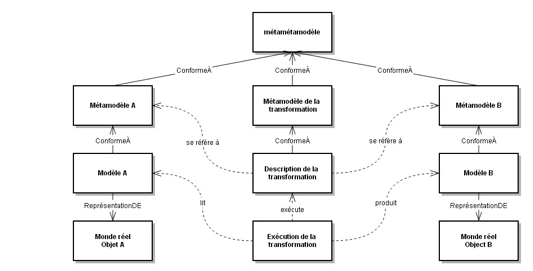
\includegraphics[width=1\textwidth]{images/Chapitre1/transfoPrincipe.png}
 \end{center}
 \caption{Méta niveaux d'une transformation de modèle}
 \label{fig:TransfoPrincipe}
\end{figure}

\subsection{Langages et outils pour la transformation de modèle}
Dans cette section, nous introduisons succinctement quelques langages et outils 
dédiés à la transformation de modèles, sans viser à l'exhaustivité.

\subsubsection{ATL}
\label{sec:ATL}
Atlas Transformation Language (ATL) \cite{jouault2006transforming} 
\cite{jouault2008atl} est né de la volonté de proposer des langages de 
modélisation dédiés à la transformation de modèle en définissant un métamodèle 
et des outils pour l'exécution des transformations. Il permet de réaliser des 
transformations de type modèle-à-modèle et de type modèle-à-texte.

ATL  est un langage hybride (déclaratif et impératif) à base de règles OCL (OMG 
2014). Une règle déclarative, appelée Matched rule, permet de décrire 
l'implémentation de mapping simples entre les modèles source et cible en 
utilisant des patrons source (\textit{InPattern}) mappés avec les éléments 
source et des patrons cibles (\textit{outPattern}) mappés avec les éléments 
cible. 

L'approche impérative explicite les étapes d'exécution de la transformation à 
travers les Helpers. Ce mécanisme de Helpers permet en outre d'éviter la 
redondance de code et la création de longues règles écrites en OCL, ce qui 
confère une meilleure lisibilité aux programmes ATL. 

Une transformation écrite en ATL est composée d'un ensemble de règles qui 
spécifient comment créer et initialiser les éléments des modèles cible. Il n'est 
pas possible de spécifier l'ordre d'exécution des règles de transformation. Cet 
ordre est établi automatiquement, exception faite pour les \textit{lazy rules} 
qui ont besoin qu'on fasse spécifiquement appel à elles. ATL est conforme au 
méta-métamodèle MOF et est doté d'une syntaxe concrète textuelle. Il est intégré 
à l'environnement Eclipse. Une transformation prend en entrée un ensemble de 
modèles conformes à Ecore (EMF 2014) ou KM3 \cite{jouault2006km3}.

ATL ne prend pas en charge les transformations incrémentales. Il commence par 
lire entièrement les modèles source et génère des modèles cible complet. Les 
modifications manuelles dans les modèles cible ne sont donc pas préservées si 
l'on opère une nouvelle transformation.

ATL peut réaliser des transformations sur  place, c'est-à-dire, une 
transformation où le modèle source et le modèle source sont confondus en 
utilisant le mode raffinement de modèle. Cependant ce mode présente quelques 
limitations avec certaines fonctionnalités comme celle des \textit{lazy rules}.

\subsubsection{QVT}
Le framework Query View Transformation (QVT) \cite{kurtev2008state} 
\cite{omg2011meta} a rejoint la batterie de standards de l'OMG. Le métamodèle de 
QVT est conforme au MOF. Comme ATL, QVT se base sur OCL pour accéder aux 
éléments des modèles.
QVT définit trois langages de transformation de type modèle-à-modèle. 
QVT-Relations (QVT-R) et QVT-Core (QVT-C) sont des langages déclaratifs qui 
adressent deux niveaux d'abstraction différents. QVT-Operational Mappings 
(QVT-OM) est un langage impératif qui étend QVT-R et QVT-C.

QVT-R est un langage de transformation de haut niveau d'abstraction doté de 
syntaxes concrètes textuelle et graphique. Les transformations, 
bidirectionnelles, sont spécifiées sous forme de relations entre les modèles 
source et cible. Une transformation a pour but de vérifier la cohérence entre 
deux modèles, renforcer la cohérence en modifiant le modèle cible, synchroniser 
deux modèles ou encore pour raffiner un modèle par une transformation sur-place. 
La sémantique de QVT-R est définie par une transformation vers QVT-C.

QVT-C est un langage de transformation de bas niveau qui sert de base pour 
QVT-R. Les deux ont le même niveau d'expressivité. Une transformation consiste 
en la déclaration de mapping entre les métamodèles source et cible en utilisant 
des patterns. Contrairement à QVT-R, la traçabilité est explicitement définie à 
travers les liens entre les métamodèles.

QVT-OM est un langage de transformation impératif qui étend QVT-R avec des 
constructions impératives basée sur une extension impérative de OCL. Les 
transformations sont unidirectionnelles mais établissent explicitement des 
modèles de traçabilité.

QVT est aussi doté d'un mécanisme de \textit{graybox} qui permet de faire appel 
à des algorithmes complexes écrits dans n'importe quel langage de programmation 
et d'utiliser des librairies existantes. Mais ce mécanisme rend la 
transformation opaque puisqu'il n'est pas contrôlé par le moteur d'exécution. 
Nous pouvons citer SmartQVT ou encore ModelMorf comme machines d'exécution de 
transformation écrite en QVT.

\subsubsection{Kermeta}
Kermeta est un langage généraliste de méta-modélisation exécutable et de 
méta-programmation orientée objet qui peut aussi décrire des transformations de 
modèle. Intégré à EMF, il est doté d'un métamodèle conforme au MOF qu'il étend 
avec un langage d'action impératif utilisé pour écrire le corps des opérations 
définies sur les concepts d'une syntaxe abstraite (ce qui revient à doter une 
syntaxe abstraite d'une sémantique opérationnelle). On peut ainsi décrire 
n'importe quel traitement sur un modèle ce qui est assimilé à une transformation 
de modèle.

Le langage d'action de Kermeta permet d'écrire des expressions impératives qui 
spécifient explicitement la construction des éléments des modèles cible. A 
l'inverse de QVT-OM, Kermeta n'est pas un langage à base de règles.  
Kermeta est capable de gérer les exceptions mais les transformations 
multidirectionnelles ne sont pas supportées par les outils d'exécution. Il en 
est de même pour la transformation incrémentale. Les modèles source sont lus en 
une seule fois et les modèles cible sont produits complets lors de l'exécution 
de la transformation.




